\documentclass[12pt]{article}
\usepackage{nips11submit_e,times}
%\RequirePackage[OT1]{fontenc}
\RequirePackage{amsbsy,amsmath,amssymb,amsthm}
\RequirePackage{graphicx}
\RequirePackage{subfigure}

\newcommand{\reals}{\mathbb{R}}
\newcommand{\trans}{\mathrm{T}}
\DeclareMathOperator*{\Tr}{Tr}
\DeclareMathOperator*{\diag}{diag}
\DeclareMathOperator*{\rank}{rank}
\newcommand{\Normal}[1][]{\mathcal{N}_{#1}}
\newcommand{\Wishart}[1][]{\mathcal{W}_{#1}}
\DeclareMathOperator*{\argmin}{argmin}

\newcommand{\prob}{\mathbb{P}}
\newcommand{\E}{\mathbb{E}}
\DeclareMathOperator*{\RSS}{RSS}

\theoremstyle{plain}
\newtheorem{theorem}{Theorem}[section]
\newtheorem{definition}[theorem]{Definition}
\newtheorem{corollary}[theorem]{Corollary}
\newtheorem{lemma}[theorem]{Lemma}
\newtheorem{proposition}[theorem]{Proposition}
\newtheorem{remark}[theorem]{Remark}




\title{
  Regularized Laplacian Estimation
  and \\ Fast Eigenvector Approximation
}
\author{
  Patrick O.~Perry \\
  School of Engineering and Applied Sciences \\
  Harvard University \\
  Harvard, MA 02138 \\
  \texttt{patperry@seas.harvard.edu} 
  \And
  Michael W.~Mahoney \\
  Department of Mathematics \\
  Stanford University \\
  Stanford, CA 94305  \\
  \texttt{mmahoney@cs.stanford.edu}
}

\newcommand{\fix}{\marginpar{FIX}}
\newcommand{\new}{\marginpar{NEW}}

%\nipsfinalcopy % Uncomment for camera-ready version

\begin{document}

\maketitle

\begin{abstract}
Recently, Mahoney and Orecchia demonstrated that popular diffusion-based 
procedures to compute a quick \emph{approximation} to the first nontrivial 
eigenvector of a data graph Laplacian \emph{exactly} solve certain 
regularized Semi-Definite Programs (SDPs). 
In this paper, we extend this result by providing a statistical 
interpretation of it.
Our interpretation will be analogous to the manner in which
$\ell_2$-regularized or $\ell_1$-regularized $\ell_2$-regression (often
called ridge regression and LASSO regression, respectively) can be
interperted in terms of a Gaussian prior or a Laplace prior, respectively,
on the coefficient vector of the regression problem.
Our framework will imply that the solutions to the Mahoney-Orecchia 
regularized SDP can be interpreted as regularized estimates of the 
pseudoinverse of the graph Laplacian.
Conversely, it will imply that the solution to this regularized estimation 
problem can be computed very quickly by running the fast diffusion-based 
PageRank procedure for computing an approximation to the first nontrivial 
eigenvector of the graph Laplacian.
Empirical results are also provided to illustrate the manner in which 
approximate eigenvector computation \emph{implicitly} performs statistical 
regularization, relative to running the corresponding exact algorithm.
\end{abstract}



\section{Introduction}
\label{sxn:intro}

Approximation algorithms and heuristic approximations are commonly used to
speed up the running time of algorithms in machine learning and data
analysis.
In some cases, the outputs of these approximate procedures are ``better''
than the output of the more expensive exact algorithms, in the sense that
they lead to more robust results or more useful results for the downstream
practitioner.
Recently, Mahoney and Orecchia formalized these ideas in the context of
computing the first nontrivial eigenvector of a graph
Laplacian~\cite{mahoney2010implementing}.
Recall that, given a graph $G$ on $n$ nodes or equivalently its $n \times n$
Laplacian matrix $L$, the top nontrivial eigenvector of the Laplacian
\emph{exactly} optimizes the Rayleigh quotient, subject to the usual
constraints.
This optimization problem can equivalently be expressed as a vector
optimization program with the objective function $f(x) = x^TLx$,
where $x$ is an $n$-dimensional vector, or as a Semi-Definite Program (SDP)
with objective function $F(X)=\mathrm{Tr}(L X)$, where $X$ is an $n \times n$
symmertic positive semi-definite matrix.
This first nontrivial vector is, of course, of widespread interest in
applications due to its usefulness for graph partitioning, image
segmentation, data clustering, semi-supervised learning, etc.~\cite{spielman96_spectral,guatterymiller98,ShiMalik00_NCut,BN03,Joa03,LLDM09_communities_IM}.

In this context, Mahoney and Orecchia asked the question: do popular
diffusion-based procedures---such as running the Heat Kernel or performing a
lazy random walk or computing the PageRank function---to compute a quick
\emph{approximation} to the first nontrivial eigenvector of $L$ solve some
other regularized version of the Rayleigh quotient objective function
\emph{exactly}.
Understanding this algorithmic-statistical tradeoff is clearly of interest
if one is interested in very large-scale applications, where performing
statistical analysis to derive an objective and then calling a black box
solver to optimize that objective exactly, might be too expensive.
Mahoney and Orecchia answered the above question in the affirmative, with
the interesting twist that the regularization is on the SDP formulation
rather than the usual vector optimization problem.
That is, these diffusion-based procedures exactly optimize the regularized
SDP $F(X)+\lambda G(X)$, for some regularization function $G(\cdot)$ to be
described below, subject to the usual constraints.

In this paper, we extend the Mahoney-Orecchia (MO) result by providing a
statistical interpretation of it.
Our interpretation will be analogous to the manner in which
$\ell_2$-regularized or $\ell_1$-regularized $\ell_2$-regression (often
called ridge regression and LASSO regression, respectively) can be
interperted in terms of a Gaussian prior or a Laplace prior, respectively,
on the coefficient vector of the regression problem.
In more detail, we will set up a sampling model, whereby the graph Laplacian
is interpreted as an observation from a random process; we will posit the
existence of a ``population Laplacian'' driving the random process; and we
will then define an estimation problem: find the inverse of the population
Laplacian.
The maximium a posteriori probability (MAP) estimate of the inverse of the
population Laplacian leads to a regularized SDP, where the objective
function $F(X)=\mathrm{Tr}(L X)$ and where the role of the penalty function
$G(\cdot)$ is to encode prior assumptions about the population Laplacian.
In addition, we show that if $G(\cdot)$ is the log-determinant function then
the MAP estimate leads to the MO regularized SDP corresponding to running
the PageRank heuristic.
Said another way, the solutions to the MO regularized SDP can be interpreted
as regularized estimates of the pseudoinverse of the graph Laplacian; and
moreover, by Mahoney and Orecchia' main result, the solution to this 
regularized SDP can be computed very quickly---rather than solving the SDP 
with a black-box solver and rather computing explicitly the pseudoinverse 
of the Laplacian, one can simply run the fast diffusion-based PageRank 
heuristic for computing an approximation to the first nontrivial eigenvector 
of the Laplacian $L$.

The next section, Section~\ref{S:introduction}, describes the background on
the Laplacian and its pseudoinverse in light of local and global versions of
the basic spectral clustering applications that gave rise to this line of
work.
Section~\ref{snx:framework} then describes a statistical framework for graph
estimation; and Section~\ref{sxn:priors} describes prior assumptions that
can be made on the population Laplacian.
These two sections will shed light on the computational implications
associated with these prior assumptions; but more importantly they will shed
light on the implicit prior assumptions associated with making certain
decisions to speed up computations.
Section~\ref{sxn:empirical} will then provide a brief empirical evaluation,
demonstrating that diffusion-based approximation algorithms for the first 
nontrivial eigenvector of the graph Laplacian implicitly leads to 
statistical regularization, relative to the corresponding exact algorithm, 
in ways that should be familiar to the reader; and Section~\ref{sxn:conc} 
will provide a brief conclusion.




\section{Background on Laplacians and local and global graph partitioning}
\label{S:introduction}

Recall that a weighted symmetric graph, $G$, is defined by a vertex set 
$V_G$, the cardinality of which 
%%%MWM%%% $V_G$, denoted $|V_G|$, 
is assumed to be finite; 
an edge set $E_G \subset V_G \times V_G$; 
and a weight function $w_G : E_G \to \reals_+$, where $w_G$ is assumed to 
be symmetric in its arguments (\emph{i.e.}, $w_G(u,v) = w_G(v,u)$).  

%%%MWM%%% I DONT THINK WE USE THE FOLLOWING PATH LENGTH DISCUSSION, BUT IT MIGHT BE GOOD TO MENTION THE NOTION OF CONNECTIVITY, BUT THAT CAN PROBABLY BE ASSUMED OF THE READER.
%%%MWM%%% A length-$l$ path in $G$, denoted $\gamma$, is defined by a finite sequence of
%%%MWM%%% vertices $\gamma(1), \gamma(2), \ldots, \gamma(l)$, where $\gamma(i) \in V_G$; given
%%%MWM%%% such a path, $\gamma(1)$ is called the start of $\gamma$ and 
%%%MWM%%% $\gamma(l)$ is called terminus of $\gamma$.  With respect to
%%%MWM%%% the graph, $G$, vertices $u$ and $v$ are said to be $l$-connected if there
%%%MWM%%% exists a length-$l$ path $\gamma$ such that $\gamma(1) = u$,
%%%MWM%%% $\gamma(l) = v$, and $w(\gamma(i), \gamma(i+1)) > 0$ for $i = 1,
%%%MWM%%% \ldots, l-1$.  Vertices $u$ and $v$ are said to be connected if they
%%%MWM%%% are $l$-connected for some positive $l$.  Connectivity defines an
%%%MWM%%% equivalence relation on the vertices of a graph.  The equivalence
%%%MWM%%% classes are called the connected components of $G$; they define a
%%%MWM%%% natural partition of the vertices.

\subsection{Global spectral partitioning}

Given a weighted symmetric graph, $G$, one can construct a positive
semidefinite matrix, $L_G \in \reals^{V_G \times V_G}$, called the 
combinatorial Laplacian of $G$:
\[
  L_G(u,v)
  =
  \begin{cases}
    - w_G(u,v) & \text{when $u \neq v$,} \\
    d_G(v) - w_G(v,v) & \text{otherwise,}
  \end{cases}
\]
where $d_G(v) = \sum_{v'} w_G(v,v')$ is called the degree of $v$.
XXX.  WE NEED TO BE CONSISTENT ABOUT COMBINATORIAL VERSUS NORMALIZED; IF WE GO WITH NORMALIZED LATER, PROBABLY BEST TO DO IT EVERYWHERE.
By construction, $L_G$ is positive semidefinite.  
Also, the all ones
vector is an eigenvector of $L_G$ with eigenvalue zero, i.e. $L_G \, 1_{V_G}
= 0$, where $1_{V_G}(v) = 1$ for all $v$; we call $1_{V_G}$ the
trivial eigenvector of $L_G$.  

If $C \subseteq V_G$ is a connected component of $G$ and 
$1_C(v) = 1\{ v \in C \}$, then $L_G \, 1_C = 0$.  
One can show that the multiplicity of the zero eigenvalue is equal to the
number of connected components in $G$.
When $G$ has exactly two connected components, say $C$ and $\bar C$,
the combinatorial Laplacian $L_G$ has two orthogonal eigenvectors
with eigenvalue $0$: the trivial eigenvector and
$c \cdot 1_C - c^{-1} \cdot 1_{\bar C}$, where
$c = \sqrt{|\bar C| / |C|}$.  
Thus, we can recover the vertex partiton
$V_G = C \sqcup \bar C$ by ``cutting'' along the first nontrivial
eigenvector of $L_G$: if $L_G x = 0$ and $1' x = 0$, then up to a sign
change in $x$, $C = \{ v : x(v) > 0 \}$ and
$\bar C = \{ v : x(v) < 0 \}$.

The idea of spectral clustering is to extend this idea to approximate the 
best partition of the vertices of a connected graph by using the nontrivial 
eigenvectors of a Laplacian (either the combinatorial Laplacian, which we 
have defined above, or a degree-normalized version).  
This idea has had a long history~\cite{Donath:1973,fiedler75B,spielman96_spectral,guatterymiller98,ShiMalik00_NCut}.
The simplest version of spectral clustering involves computing the first 
nontrivial eigenvector (or another vector with Rayleigh quotient close to 
that of the first nontrivial eigenvector) of $L_G$, and ``sweeping'' over 
that vector. 
For example, 
%%%MWM%%% to partition the vertices into two sets, 
one can take that vector, call it $x$, and, for a given threshold $K$, 
define the two sets of the partition as
\begin{align*}
  C(x,K)      &= \{ i : x_i >= K \}, \quad \text{and} \\
  \bar C(x,K) &= \{ i : x_i < K \}.
\end{align*}
%%%MWM%%% Importantly, procedure defines a partion even when the vertices of $G$ are 
%%%MWM%%% all connected.  
XXX.  CITE FIRST FIG HERE, BUT PROBABLY HAVE A FIRST SUBFIG THAT GIVES THE USUAL 50-50 SPLIT AS WELL.
Typically, this vector is computed by calling a black-box solver, but it 
could also be approximated with an iteration-based method (such as the Power
Method or Lanczos Method) or a random walk-based method (such as running a 
diffusive procedure or PageRank-based procedure to the asymptotic state).
Far from being a heuristic, this procedure provides a \emph{global 
partition} that (via Cheeger's inequality and for an appropriate choice of 
$K$) satisfies provable quality-of-guarantees with respect to the 
combinatorial problem of finding the best ``conductance'' partition in the 
entire graph~\cite{Mihail,spielman96_spectral,guatterymiller98}.

\begin{figure}
    \centering
    \makebox{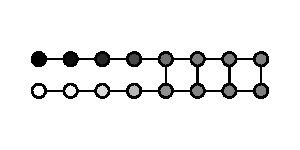
\includegraphics[scale=0.8]{plots/guattery-global}}
    \caption{
             Global partition from first nontrivial eigenvector of the Laplacian.
XXX.  MAYBE TWO SUBFIGURES, ONE FOR A GRAPH WITH A GOOD BIPARTITION WHERE SPECTRAL WORKS AND THE GUATTERY ONE WHERE IT DOESNT.
}
\end{figure}


\subsection{Local spectral partitioning}

If spectral clustering reduces a graph to a single vector---the smallest
nontrivial eigenvector of the graph's Laplacian---and then clusters the 
nodes using the information in the vector, it is possible to obtain much 
more information about the graph by looking at more than one eigenvector 
from the Laplacian.  
In particular, the elements of the pseudoinverse of the Laplacian give 
local (\emph{i.e.}, node-specific) information about random
walks on the graph.
The reason is that if $G$ is a graph with combinatorial Laplacian $L_G$, 
then the pseudoinverse $L_G^+$  of the Laplacian is closely related to 
random walks on the graph.  
In particular, $L_{G}^{+}$ defines a proximity measure on the graph with the
following properties:
\begin{description}
  \item[Symmetry]
    $L_G^{+}(u,v) = L_G^{+}(v,u)$;
 \item[Diagonal maximality]
    $L_G^{+}(u,u) > L_G^{+} (u,v)$ whenever $u \neq v$;
  \item[Triangle inequality for proximities]
    If $u$ and $v$ are in the same connected component, then
    $L_G^{+} (u,v) + L_G^{+} (u,w) - L_G^{+} (v,w) \leq L_G^{+} (u,u)$, with strict inequality
    holding when $v = w$ and $u \neq v$;
  \item[Metric representability]
   $L_G^{+} (u,u) + L_G^{+} (v,v) - L_G^{+} (u,v) - L_G^{+} (v,u)$
    defines a metric on every connected component of $V_G$;  this is commonly called
    \emph{resistance distance} on $G$.
 \item[Transit property]
    if $G$ contains a path from $u$ to $v$, and each path from $u$ to
    $v$ includes $w$, distinct from $u$ and $v$, then $L_G^{+}(u,w) >
    L_G^{+}(u,v)$.
\end{description}
See, \emph{e.g.}~\cite{chebotarev1998proximity} for details.  
%%%MWM%%% A full discusion of this
%%%MWM%%% These properties follow from Chebotarev and Shamis' topological
%%%MWM%%% representation of of the combinatorial Laplacian
%%%MWM%%% \cite{chebotarev1998proximity}.  A full discusion of this
%%%MWM%%% representation is beyond the scope of the present treatment, but for
%%%MWM%%% unweighted, connected graphs, the authors show that if $|V_G| = n$,
%%%MWM%%% then
%%%MWM%%% \[
%%%MWM%%%   L_G^{+}(u,v) = \frac{|\mathcal{F}_{n-2}^{uv}| - \frac{1}{n}
%%%MWM%%%     \sum_{w} |\mathcal{F}_{n-2}^{uw}|}{|\mathcal{F}_{n-1}|},
%%%MWM%%% \]
%%%MWM%%% where $\mathcal{F}_k$ and $\mathcal{F}_k^{uv}$ are sets of subgraphs
%%%MWM%%% of $G$; the set $\mathcal{F}_{k}$ comprises all rooted spanning forests
%%%MWM%%% with $k$ edges, and $\mathcal{F}_{k}^{uv}$ comprises all rooted spanning
%%%MWM%%% spanning forests with $k$ edges such that $u$ is a root, and $v$
%%%MWM%%% belongs to the same tree as $u$.  
In addition, it is known that the
%%%MWM%%% Chandra et al.\ show that the
quantity $L_G^{+} (u,u) + L_G^{+} (v,v) - L_G^{+} (u,v) - L_G^{+} (v,u)$ is
proportional to the length of time before a random walker started at
node $u$ reaches node $v$ whenever $u$ and $v$ are in the same
connected component~\cite{chandra1989electrical}.  
%%%MWM%%% It is likely that $L_G^{+}(u,v)$ has a probabalistic interpretation in terms 
%%%MWM%%% of random walks on the graph, but we are not aware of any such 
%%%MWM%%% interpretation.

From this perspective, given $L_G^{+}$ and a cutoff value, $K$, we can 
define a \emph{local partition} around node $u$ via 
$P_K(u) = \{ v : L_G^{+}(u,v) > K \}$.  
(Note that if $v$ is in $P_K(u)$, then $u$ is in $P_K(v)$.  In addition, in 
light of the disconnection condition, if the graph is disconnected, then 
there exists a $K$ such that $u$ and $v$ are in the same connected component 
iff $v \in P_K(u)$.)  
We call this partitioning \emph{local spectral clustering}.
Although the na\"{i}ve way of performing this partitioning, \emph{i.e.}, to 
compute $L_G^{+}$ explicitly, is prohibitive for anything but very small 
graphs, these ideas form the basis for very fast local spectral clustering 
methods that truncated diffusion-based procedures to compute localized 
vectors with which to partition; 
see~\cite{Spielman:2004,andersen06local,Chung07_heatkernelPNAS,MOV09_TRv2} 
for details.

\begin{figure}
    \centering
    \makebox{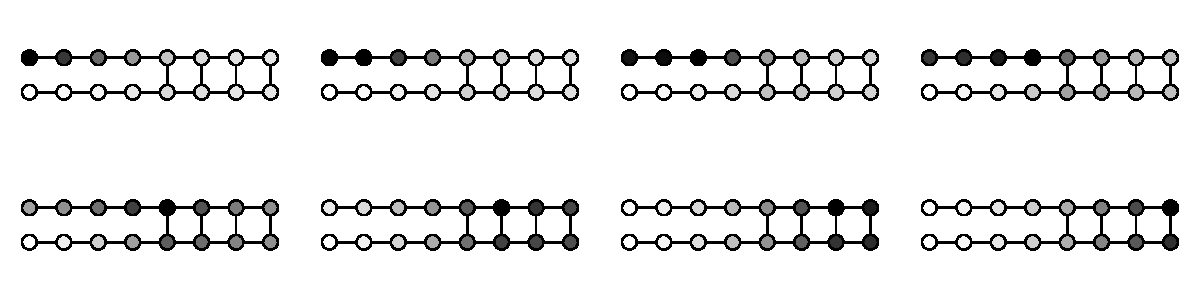
\includegraphics[scale=0.6]{plots/guattery-local}}
    \caption{Local partitions from the pseudoinverse of the Laplacian}
\end{figure}
\begin{figure}
    \centering
    \makebox{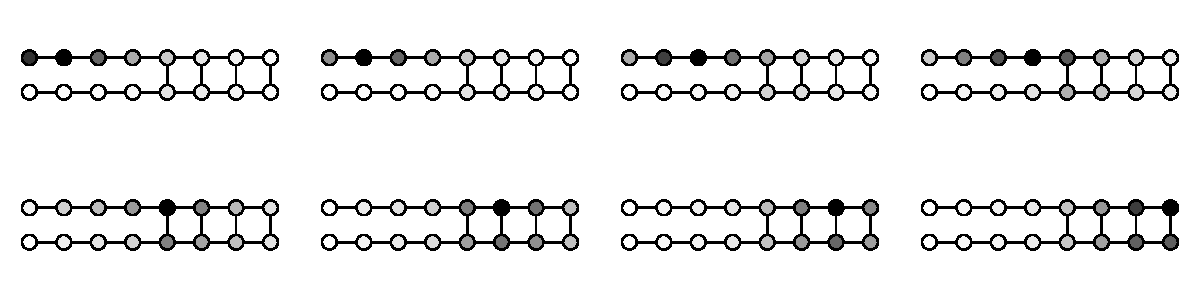
\includegraphics[scale=0.6]{plots/guattery-pagerank}}
    \caption{Local partitions from PageRank}
\end{figure}

[Add Guattery example here, showing benefits of local spectral.]


\subsection{Approximating local and global spectral partitioning with 
diffusion-based procedures}

Of course, the pseudoinverse of the Laplacian is seldom (if ever) used to 
partition the nodes of a graph.
Moreover, in certain cases, one might not call a black-box solver to comptue 
the smallest nontrivial eigenvector of Laplacian exactly.
In both of these cases, an extension to the basic spectral clustering 
involves running procedures based on random walks or diffusions 
%%%MWM%%% (started with a random vector or a deterministic vector with all 
%%%MWM%%% of its mass localized on one or a small number of seed nodes) 
on the graph.  
These approaches assign positive and negative ``charge'' to the nodes,
and then let the distribution of charge evolve according to dynamics
derived from the graph structure.
(Three variants may be found in recent work on local spectral graph 
partitioning~\cite{Spielman:2004,andersen06local,Chung07_heatkernelPNAS}.)
Three canonical evolution dynamics are the following.
\begin{description}
  \item[Heat Kernel.]
    Here, the charge evolves according to the dynamics of the heat equation
    $\frac{\partial H_t}{\partial t} = - L_G H_t$.
    Thus, the vector of charges evolves as
    \begin{equation}
    \label{eqn:heat-kernel}
    H_t = \exp ( -tL )  = \sum_{k=0}^{\infty} \frac{(-t)^k}{k!}L^k  ,
    \end{equation}
    where $t \ge 0$ is a time parameter, times an input seed distribution.
  \item[PageRank.]
    Here, the charge at a node evolves by either moving to a neighber of 
    the current node or teleporting to a random node.
    More formally, then the vector of charges evolves as 
    \begin{equation}
    \label{eqn:page-rank}
    R_{\gamma} = \gamma \left(I-\left(1-\gamma \right)M \right)^{-1}   ,
    \end{equation}
    where $M$ is the natural random walk transition matrix associated 
    with the graph and
    where $\gamma \in (0,1)$ is the so-called teleportation parameter,
    times an input seed distribution.
  \item[Lazy Random Walk.]
    Here, the charge either stays at the current node or moves to a neighbor.
    Thus, if $M$ is the natural random walk transition matrix associated 
    with the graph, then the vector of charges evolves as some power of 
    \begin{equation}
    \label{eqn:lazy-walk}
    W_{\alpha}= \alpha I + (1-\alpha)M ,
    \end{equation}
    where $\alpha \in (0,1)$ represents the ``holding probability,'' times 
    an input seed distribution.
\end{description}
In each of these cases, there is a parameter ($t$, $\gamma$, and the number 
of steps of the lazy random walk) that controls the ``aggressiveness'' of 
the dynamics and thus controls how quickly the diffusive process 
equilibrates; and there is an input seed distribution.
If one is interested in global spectral partitioning, then this seed vector 
could be a vector with entries drawn from $\{-1,+1\}$ uniformly at random, 
while if one is interested in local spectral partitioning, then this vector 
could be the indicator vector of a small ``seet set'' of nodes.

In either case, Mahoney and Orecchia showed that these three dynamics arise 
as solutions to regularized SDPs of the form
\begin{equation}
\begin{aligned}
  & \underset{X}{\text{minimize}}
  & & \mathrm{tr}(L_G X) + \lambda G(X) \\
  & \text{subject to}
  & & X \succeq 0, \\
  & & & \mathrm{tr}(X) = 1, \\
  & & & \mathrm{tr}(X J) = 0,
\end{aligned}
\label{eqn:mo-reg-sdp}
\end{equation}
where $J = 1_{V_G} 1_{V_G}'$ and $G$ is a penalty function (generalized 
entropy, log-determinant and a certain matrix-$p$-norm, 
respectively~\cite{mahoney2010implementing}) and where $\lambda$ is a 
parameter related to the aggressiveness of the diffusive 
process~\cite{mahoney2010implementing}.  
Notably, when $G = 0$, the solution to the SDP 
of~(\ref{eqn:mo-reg-sdp}) is $u u'$, where $u$ is the smallest nontrivial 
eigenvector of $L_G$.  
More generally, in this precise sense, the heat kernel, PageRank, and lazy 
random walk dynamics can be seen as ``regularized'' versions of spectral 
clustering and Laplacian eigenvector computation.
XXX.  MWM CHANGED REGULARIZATION FXN FROM $F$ TO $G$ TO BE CONSISTENT WITH BEFORE, WEN NEED TO BE CONSISTENT EVERYWHERE.
Intuitively, where the function $G(\cdot)$ is acting as a penalty function, 
in a manner analogous to the $\ell_2$ or $\ell_1$ penalty in ridge 
regression or LASSO.
In this paper, we provide a statistical framework to make that intuition 
precise.

%%%MWM%%% In the sequal, we extend Mahoney and Orecchia's
%%%MWM%%% result, showing that solutions to the regularized SDP can be
%%%MWM%%% interpreted as regularized estimates of the pseudoinverse of the
%%%MWM%%% Laplacian.  Specifically, we set up a sampling model, whereby the
%%%MWM%%% Laplacian is interpreted as an observation from a random process.  We
%%%MWM%%% posit the existence of a ``population Laplacian'' driving the random
%%%MWM%%% process.  We then define an estimation problem: finding the inverse of
%%%MWM%%% the population Laplacian.  It turns out that the solution to the
%%%MWM%%% regularized SDP arrises as the maximium a posteriori probability (MAP)
%%%MWM%%% estimate of the inverse of the population Laplacian.  The role of the
%%%MWM%%% penalty function, $F$, is to encode prior assumptions about the
%%%MWM%%% population Laplacian.

(((
XXX.  INCORPORATE WITH SUBSXN BELOW OR REMOVE IF REDUNDANT.
Our approach is reminiscent of the Bayesian interpretation of
regularized linear regression.  In linear regression, an $L^2$ penalty
corresponds to a Gaussian prior on the coefficent vector, and the
solution to the regularized regression problem is the maximium a
posterior (MAP) estimator.  In the same setting, $L^1$ regularization
corresponds to a Laplace prior on the coefficent vector.
)))


\section{A statistical framework for regularized graph estimation}
\label{snx:framework}

Here we lay out a simple Bayesian framework for estimating a graph
Laplacian, which allows for regularization by incorporating prior
information.  We suppose that the observed graph Laplacian, $L$, is a
random object whose distrubution depends on a true ``population''
Laplacian, $\mathcal{L}$.  This induces a conditional density for $L$,
denoted $p(L \mid \mathcal{L})$.  Next, we assume prior information
about the population Laplacian in the form of a prior density,
$p(\mathcal{L})$.  Given the observed Laplacian, we estimate the
population Laplacian by maximizing its posterior density,
$p(\mathcal{L} \mid L)$.


\subsection{Analogy with regularized linear regression}\label{S:regression}

It will be helpful to keep in mind the Bayesian
interpretation of regularized linear regression.  In that context, we
observe $n$ predictor-response pairs in $\reals^p \times \reals$,
denoted $(x_1, y_1), \dotsc, (x_n, y_n)$; the goal is to find a vector
$\beta$ such that $\beta' x_i \approx y_i$.  Typically, we choose
$\beta$ by minimizing the residual sum of squares,
$\RSS(\beta) = \sum_i \| y_i - \beta' x_i \|_2^2$, or a
penalized version of it.  For ridge regression, we minimize
$\RSS(\beta) + \lambda \|\beta\|_2^2$; for LASSO regression, we minimize
$\RSS(\beta) + \lambda \|\beta\|_1$.  The additional terms in the
optimization criteria ($\lambda \|\beta\|_2^2$ and $\lambda
\|\beta\|_1$) are called penalty functions.

Adding a penalty function to the optimization criterion can be
interpreted as incorporating prior information about $\beta$.  We
model $y_1, \dotsc, y_n$ as independent random observations with
distributions dependent on $\beta$.  Specifically, we suppose $y_i$ is
a Gaussian random variable with mean $\beta' x_i$ and known variance
$\sigma^2$.  This induces a conditional density for the vector
$y = (y_1, \dotsc, y_n)$:
\begin{equation}\label{E:regression-density}
  p(y \mid \beta)
    \propto
     \exp\{ -\tfrac{1}{2 \sigma^2} \RSS(\beta) \},
\end{equation}
where the constant of proportionality depends only on $y$ and $\sigma$.
Next, we assume that $\beta$ itself is random, drawn from a
distribution with density $p(\beta)$.  This distribution is called a
prior, since it encodes prior knowledge about $\beta$.  Without loss
of generality, the prior density can be assumed to take the form
\begin{equation}\label{E:regression-prior}
  p(\beta) \propto \exp\{ -\tfrac{1}{2} F(\beta) \}.
\end{equation}
Since the two random variables are dependent, upon observing $y$, we
have information about $\beta$.  This information is incoded in the
posterior density, $p(\beta \mid y)$, computed via
Bayes' rule as
\begin{equation}\label{E:regression-posterior}
  p(\beta \mid y)
    \propto p(y \mid \beta) \, p(\beta)
    \propto \exp\{ -\tfrac{1}{2 \sigma^2} \RSS(\beta) - \tfrac{1}{2} F(\beta) \}.
\end{equation}
The maximum a posterior probablility (MAP) estimate of $\beta$ is the
value that maximizes $p(\beta \mid y)$.  Equivalently, $\beta$
minimizes $\log p(\beta \mid y)$.  We can recover the solution to
Ridge or LASSO regression by setting
$F(\beta) = \tfrac{\lambda}{\sigma^2} \| \beta \|_2^2$ or
$F(\beta) = \tfrac{\lambda}{\sigma^2} \| \beta \|_1$.  Thus, Ridge
regression can be interpeted as imposing a Gaussian prior on $\beta$,
and LASSO regression can be interpreted as imposing a
double-exponential prior on $\beta$.


\subsection{Bayesian inference for the population Laplacian}
\label{S:bayesian-laplacian}

Suppose $L$ is the normalized Laplacian of a connected graph with $n$
nodes.  Take $L$ to be a random object with expectation~$\mathcal{L}$,
where $\mathcal{L}$ is another normalized graph Laplacian.  We refer to $\mathcal{L}$ as the
``population'' graph Laplacian, and we refer to $L$ as the ``sample''
graph Laplacian.  In general, $\mathcal{L}$ can be distinct from $L$,
but we require that the nodes in the population and sample graphs have
the same degrees, given by the vector $d = \big(d(1), \dotsc,
d(n)\big)$. Let $D = \diag\big(d(1), \dotsc, d(n)\big)$ and let
$\mathcal{X} = \{ X : X \succeq 0, \, X D^{1/2} 1 = 0, \, \rank(X) = n - 1 \}$.  The
population and sample Laplacians are both members of $\mathcal{X}$.


To apply the Bayesian formalism, we need to fully specify the
conditional density of $L$ given $\mathcal{L}$.  In
Sec.~\ref{S:regression}, in the context of linear regression, we
assumed that the observations followed a Gaussian distrubition.  A
graph Laplacian is not a single observation---it is a positive
semidefinite matrix with a very specific structure.  To model $L$, we
choose a distribution for positive semi-definite matrices analogous to
the Gaussian distribution: a scaled Wishart matrix with expectation
$\mathcal{L}$.  This distribution captures the trait that $L$ is
positive semi-definite.  The distribution does not accurately model
every feature of $L$, in particular a scaled Wishart matrix does not
necessarily have ones along its diagonal.  However, the mode of the
density is at $\mathcal{L}$, a Laplacian, and for large values of the
scale parameter, most of the mass will be on matrices close to
$\mathcal{L}$.

Let $m \geq n - 1$ be a scale parameter
and suppose $L$ is distributed as a
$\tfrac{1}{m} \mathrm{Wishart}(\mathcal{L}, m)$ random variable.
Thus, $\E[L \mid \mathcal{L}] = \mathcal{L}$ and $L$ has conditional density
\begin{equation}\label{E:density}
  p(L \mid \mathcal{L})
    \propto
      \frac{\exp\{ -\frac{m}{2} \Tr(L \mathcal{L}^+)\}}
           {|\mathcal{L}|^{m/2}},
\end{equation}
where $|\cdot|$ denotes pseudodeterminant (product of nonzero
eigenvalues).  The constant of proportionality depends only on $L$,
$d$, $m$, and $n$, and the density is supported on $\mathcal{X}$.
Eq.~\eqref{E:density} is analogous to Eq.~\eqref{E:regression-density}
in the linear regression context, with $1/m$ playing the role of
$\sigma^2$.

Now suppose we have know that $\mathcal{L}$, is a random object drawn
from a prior density $p(\mathcal{L})$.
Without loss of generality,
\begin{equation}\label{E:prior}
  p(\mathcal{L}) \propto \exp\{ -\tfrac{1}{2} \tilde G(\mathcal{L}^+) \},
\end{equation}
for some function $F$, supported on a subset
$\mathcal{S} \subseteq \mathcal{X}$.  (The space $\mathcal{X}$ is
closed under inversion, so if $\mathcal{L}^{+} \in \mathcal{S}$, then
$\mathcal{L} \in \mathcal{X}$.)
Eq.~\eqref{E:prior} is analogous to Eq.~\eqref{E:regression-prior}.

Upon observing $L$, the posterior distribution for $\mathcal{L}$ is
\begin{equation}\label{E:posterior}
  p(\mathcal{L} \mid L)
    \propto p(L \mid \mathcal{L}) \, p (\mathcal{L})
    \propto \exp\{ -\tfrac{m}{2} \Tr(L \mathcal{L}^+)
                   + \tfrac{m}{2} \log |\mathcal{L}^+|
                   - \tfrac{1}{2} F(\mathcal{L^+}) \},
\end{equation}
with support determined by $\mathcal{S}$.  Eq.~\eqref{E:posterior} is
analogous to Eq.~\eqref{E:regression-posterior}.  The MAP estimator of
$\mathcal{L}$ is the pseudoinverse of the solution to the program
\[
\begin{aligned}
  & \underset{X}{\text{minimize}}
  & & \Tr(L X) + \tfrac{1}{m} F(X) - \log |X| \\
  & \text{subject to}
  & & X \in \mathcal{S}.
\end{aligned}
\]
Note the similarity with Mahoney and Orecchia's relaxed SDP.
In particular, if
\(
  \mathcal{S} = \{ X : \Tr(X) = 1 \} \cap \mathcal{X},
\)
then the two programs are identical except for the factor of
$\log |X|$ in the optimization criterion.  Prop~\ref{P:map-sdp} makes
this connection precise.

%More generally, if 
%$\mathcal{S} = \{ X : \Tr(X) = \tau^{-1} \} \cap \mathcal{X}$, then
%the MAP estimator of
%$[\Tr(\mathcal{L}^{+})]^{-1} \mathcal{L}^{+} = \tau \mathcal{L}^+$ is
%the solution to the program
%\[
%\begin{aligned}
%  & \underset{X}{\text{minimize}}
%  & & \Tr(L X) + \tfrac{\tau}{m} F(\tau^{-1} X) - \tau \log |X| \\
%  & \text{subject to}
%  & & X \succeq 0 \\
%  & & & X D^{1/2} 1 = 0 \\
%  & & & \Tr(X) = 1
%\end{aligned}
%\]


\section{Prior}
\label{sxn:priors}

To successfully leverage the results in the preceding section, we need
to choose densities $p(\mathcal{L})$ that encode our prior beliefs in
particular application regimes.  In this section, we present a
parametric form for the prior that allows us to interpolate between
``expander-like'' graphs and ``low-dimensional'' graphs.  For a
network to be expander-like, we expect the gaps between consecutive
eigenvalues of the Laplacian to be small.  For a network to be
low-dimensional, we expect the smallest non-trivial eigenvalues to be
well-separated from the rest of the spectrum (simulations in
Sec.~\ref{sxn:empirical} formalize this intuition).
Secs.~\ref{S:prior-support}--\ref{S:prior-density} define a
parametric family of priors for $\mathcal{L}$, and
Sec.~\ref{S:posterior-density} develops the corresponding posterior
density for $\mathcal{L}$ and its maximizer.

XXX.  I THINK WE SHOULD DO THINGS IN THE REVERSE ORDER.  THAI IS, I THINK WE SHOULD SAY THAT WE WANT PRIORS THAT CORRESPOND TO THE MO-REGULARIZED-SDP; THEN JUST GIVE THEN AND SHOW WHAT SDPS WE GET; THEN SAY FOR HEAT KERNEL AND LAZY WALK WE ARE ALMOST THERE BUT FOR PAGERANK WE GET EXACTLY WHAT WE HAD BEFORE; AND ONLY THEN DRAW CONNECTIONS TO LOW-DIM AND EXPANDERS, INCLUDING WHY IN TERMS OF SOCIAL GRAPHS THAT IS OF INTEREST AND A DISCUSSION OF THE ANALYTICAL AND EMPIRICAL PRIORS.  AND THEN MOVE ONTO THE EMPIRICAL RESULTS SECTION.  I THINK IT MAKES MORE SENSE IN TERMSOF LOCICAL FLOW AND RIGOR.

\subsection{Prior support set}
\label{S:prior-support}

The prior is supported on a subset of positive-semidefinite
matrices.  The support set is $\mathcal{X}$, the same support set, as
for the conditional density defined in
Sec.~\ref{S:bayesian-laplacian}, so that every matrix in the support
set is positive semi-definite, has rank $n - 1$, and satisfies
$X D^{1/2} 1 = 0$.


\subsection{Prior density}
\label{S:prior-density}

The prior we specify depends only on the eigenvalues of the normalized
Laplacian.  Equivalently, it depends only on the eigenvalues of the pseudoinverse of
the Laplacian.  If $\mathcal{L}^+ = \tau \, U \Lambda U'$ is the spectral
decomposition of the pseudoinverse of normalized Laplacian
$\mathcal{L}$, where $\tau \geq 0$,
$U \in \reals^{n \times n -1}$, 
$\Lambda = \diag\big(\lambda(1), \dotsc, \lambda({n-1})\big)$, and
$\sum_v \lambda(v) = 1$,  then the prior
weight on $\mathcal{L}$ only depends on $\tau$ and $\Lambda$.  Note that the
values $\lambda(1), \dotsc, \lambda(n-1)$ are unordered.

The implication is that the prior is ``nearly'' rotationally
invariant, i.e. $p(O \mathcal{L} O') = p(\mathcal{L})$ for any rank-$(n-1)$
projection matrix $O$ satisfying $O' D^{1/2} 1 = 0$.

The vector $\lambda = \big(\lambda(1), \dotsc, \lambda(n-1)\big)$ lies
in the unit simplex.  If we require that the
distribution for $\lambda$ be exchangeable (invariant under
permutations) and neutral ($\lambda(v)$ independent of the vector
$\big(\lambda(u) / (1 - \lambda(v)) : u \neq v\big)$ for all $v$),
then the only non-degenerate possibility is that $\lambda$ is
Dirichlet-distributed with parameter vector $(\alpha, \ldots, \alpha)$
\cite{fabius1973two}.  The parameter $\alpha$, which we refer to as
the ``shape'' parameter, must satisfy $\alpha > 0$ for the density to
be defined.  In this case,
\begin{equation}\label{E:dirichlet-prior}
  p(\mathcal{L})
   \propto p(\tau) \prod_{v=1}^{n-1} \lambda(v)^{\alpha - 1},
\end{equation}
where $p(\tau)$ is a prior for $\tau$.

In Fig~\ref{F:dirichlet}, we display the behavior of the order
statistics of $\lambda$ as $\alpha$ varies.  We fix the value $n = 42$
and then let $\alpha$ vary between $0.2$ and and $2$.  For each value
of the shape $\alpha$, we generate a random $(n-1)$-dimensional Dirichlet
vector, $\lambda$, with parameter vector $(\alpha, \dotsc, \alpha)$.
We compute the $n-1$ order statistics of $\lambda$ by sorting its
components.  We repeat the procedure for $500$ replicates and then
average the values.  For small values of $\alpha$, we observe that the
first few order-statistics are well-separated from the rest.  As
$\alpha$ increases, the order statistics become concentrated
around $1/(n-1)$.

\begin{figure}
    \centering
    \subfigure[Dirichlet distriubtion order statistics]{
      \makebox{\label{F:dirichlet}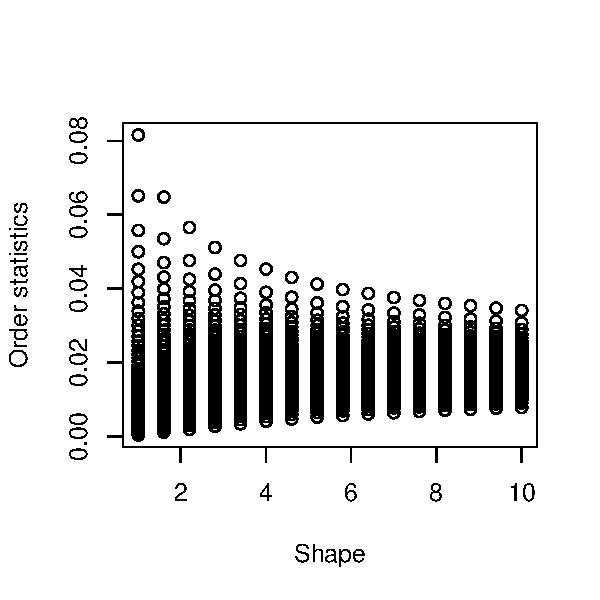
\includegraphics[scale=0.6]{plots/dirichlet}}
    }
    \subfigure[Interpolating from a low-dimensional graph to an expander]{
      \makebox{\label{F:interpolate}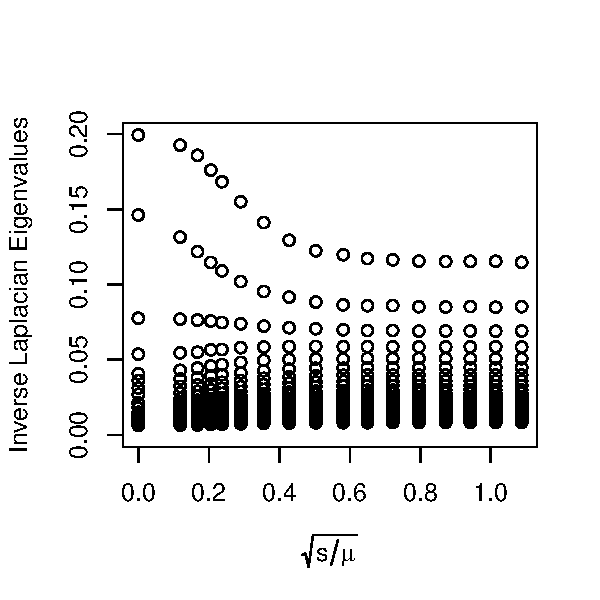
\includegraphics[scale=0.6]{plots/interpolate}}
    }
    %\caption{Analytical and emprical priors}
\end{figure}



\subsection{Posterior estimation and connection to PageRank}
\label{S:posterior-density}

\begin{proposition}\label{P:map-sdp}
  Suppose the conditional likilihood for $L$ given $\mathcal{L}$ is as
  defined in \eqref{E:density} and the prior density for $\mathcal{L}$
  is as defined in \eqref{E:dirichlet-prior}.  If
  $\mathcal{\hat L}$ is the MAP estimate of $\mathcal{L}$, then
  there exists an $\eta$ such that
  $[\Tr(\mathcal{\hat L}^+)]^{-1} \mathcal{\hat L}^+$ solves the
  Mahoney-Orecchia SDP \eqref{eqn:mo-reg-sdp} with $G(X) = -\log |X|$.
\end{proposition}

\begin{proof}
For $\mathcal{L}$ in the support set of the posterior,
define $\tau = \Tr(\mathcal{L}^+)$ and $\Theta  = \tau^{-1}
\mathcal{L}^+$, so that $\Tr(\Theta) = 1$.  Further, $\rank(\Theta) = n - 1$.
Express the prior in the form of Eq.~\eqref{E:prior} with function
$\tilde G$ given by
\[
  \tilde G(\mathcal{L}^+)
    = -2 \log \{ p(\tau) \, |\Theta|^{\alpha - 1} \}
    = -2(\alpha - 1) \log |\Theta| - 2 \log p(\tau),
\]
where as before, $|\cdot|$ denotes pseudodeterminant.  Using
\eqref{E:posterior} and the relation
$|\mathcal{L}^+| = \tau^{n-1} |\Theta|$, the posterior
density for $\mathcal{L}$ given $L$ is
\[
  p(\mathcal{L} \mid L)
    \propto
      \exp\Big\{
        -\tfrac{m \tau}{2} \Tr(L \Theta)
        +\tfrac{m + 2(\alpha - 1)}{2} \log | \Theta |
        + g(\tau)\Big\},
\]
where
\(
  g(\tau)
    = \tfrac{m (n-1)}{2} \log \tau
        + \log p(\tau).
\)
Suppose $\mathcal{\hat L}$ maximizes the
posterior likelihood.  Define $\hat \tau = \Tr(\mathcal{\hat L}^+)$
and $\hat \Theta = [\hat \tau]^{-1} \mathcal{\hat L}^{+}$.
In this case, $\hat \Theta$ must minimize the quantity
\(
  \Tr(L \hat \Theta) - \tfrac{1}{\eta} \log |\hat \Theta|,
\)
where
\begin{equation}\label{E:eta}
  \eta
    = \frac{m \hat \tau}{m + 2(\alpha - 1)}.
\end{equation}
Thus $\hat \Theta$ solves \eqref{eqn:mo-reg-sdp} with $G(X) = - \log |X|$.
\end{proof}

Mahoney and Orecchia showed that the solution to
\eqref{eqn:mo-reg-sdp} with $G(X) = - \log |X|$
is closely related to the PageRank matrix, $R_\gamma$.  Combining
Prop.~\ref{P:map-sdp} with their result, we get that the MAP estimate
of $\mathcal{L}$ satisfies
\(
  \mathcal{\hat L}^+
    \propto D^{-1/2} R_\gamma D^{1/2};
\)
conversely,
\[
  R_\gamma
    \propto
      D^{1/2} \mathcal{\hat L}^+ D^{-1/2}.
\]
Thus, the PageRank matrix
can be viewed as a degree-scaled regularized estimate of the
pseudoinverse of the Laplacian.


\section{Empirical evaluation}
\label{sxn:empirical}

Here, we evaluate the performance of the regularized Laplacian
estimator compared to the unregularized estimator.

\subsection{Prior evaluation}\label{S:prior-evaluation}

First, we evaluate the prior.  In our setup, we start two-dimensional
lattice with width $w$ and height $h$, and $n = w h$ nodes.  Points in
the lattice are connected to their four nearest neighbors, except on
the boundary.  We then perform $s$ edge-swaps: for each swap, we
choose two edges uniformly at random and then we swap the endpoints.
(For example, if we sample $i_1 \sim j_1$ and $i_2 \sim j_2$, then we
replace these edges with $i_1 \sim j_2$ and $i_2 \sim j_1$.)  By
varying the number of swaps, we interpolate between a low-dimensional
graph and an expander.

For each value of $s$, we generate the normalized Laplacian, $\mathcal{L}$,
corresponding to the random $s$-swapped grid.  We compute the $n-1$ nonzero
eigenvalues of $[\Tr(\mathcal{L}^{+})]^{-1} \mathcal{L}^{+}$.
Finally, we perform $1000$ replicates of the procedure and average the
resulting eigenvalues.  Fig.~\ref{F:interpolate} shows the results of
the simulation.  We can see that when $s = 0$, the top two eigenvalues
(corresponding to the width-wise and height-wise coordinates on the grid)
are well separated from the bulk.  As we increase $s$, the top eigenvalues
merge into the bulk; eventually, as $s$ goes to infinity, the
distribution will be very close that that of a uniformly chosen
$4$-regular graph.


\subsection{Estimation performance}\label{S:estimation}

Next, we evaluate the estimation performance of a regularized
estimator of the graph Laplacian as compared to an unregularized
estimate.

To evaluate the performance, we need a ground truth and a noisy
observation.  To construct such a pair, we generate population graph
$\mathcal{G}$ with Laplacian $\mathcal{L}$ as in
Sec.~\ref{S:prior-evaluation}, using width $w = 7$, height $h = 6$,
and edge-swaps $s = 4$.  This will be the ground truth.  We define
$\tau = \Tr(\mathcal{L}^+)$ and $\Theta = \tau^{-1} \mathcal{L}^+$;
the goal will be to estimate $\Theta$.  As above, we let $n = w h$,
the number of nodes in the graph.

Next, we generate a noisy observation.  We randomly choose $m$ edges
with replacement from $\mathcal{G}$.  We define sample graph $G$
and corresponding Laplacian by setting the weight of $i \sim j$
to the number of times we sampled that edge.  Finally we set
$t = \Tr(L^+)$ and $O = t^{-1} L^+$.  The matrix $O$ is the
unregularized estimate of $\Theta$.  In our experiment, we set $m = n$.

For a given value of the regularization parameter, $\eta$, we compute
$\hat \Theta_\eta$, an estimate of $\Theta$, by solving the
Mahoney-Orecchia SDP with $G(X) = -\log|X|$.  Our performance measure
is relative Frobenius error, $\| \hat \Theta_\eta - \Theta \|_\mathrm{F} / \| O - \Theta
\|_\mathrm{F}$, where $\| \cdot \|_\mathrm{F}$ denotes Frobenius norm
($\|A\|_\mathrm{F}^2 = \Tr(A' A)$).  In the supplementary materials,
we also look at relative spectral error, replacing Frobenius norm with
spectral norm; the results are qualitatively similar.


In Fig.~\ref{F:estimation-frob}, we generate $100$ ground truth/noisy
observation pairs according to the procedure just described.  For each
replicate, we sweep over values of $\eta$ and evaluate the relative
Frobenius error.  The figure shows mean relative Frobenius error and
one standard devation around it plotted as a function of
$\eta / \bar \tau$, where $\bar \tau$ is the mean value of $\tau$
(compare with \eqref{E:eta}).  Regularization shows an improvement
over the naive estimate of $\Theta$ for many values of $\eta$.  In the
supplementary materials, we show that this behavior persists as we
vary $m$, with smaller values of $m$ corresponding to larger benefits
from regularization.



\subsection{Optimal regularization behavior}

The optimal amount of regularization depends on the population graph
and the sampling procedure.  Continuing with the simulation of
Sec.~\ref{S:estimation}, we investigate how the optimal value of
$\eta$ varies with $s$ and $m$.


\begin{figure}
    \centering
    \subfigure[Relative Frobenius error versus $\eta / \bar \tau$]{
      \makebox{\label{F:estimation-frob}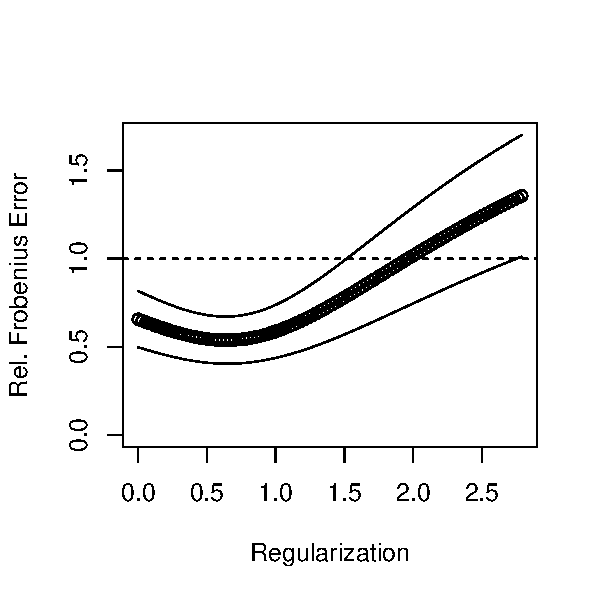
\includegraphics[scale=0.6]{plots/estimation-frob-p100}}
    }
    \subfigure[Scaled optimal regularization parameter $\eta / \bar \tau$ plotted against $m$
    and $s$]{
      \makebox{\label{F:optimal-frob}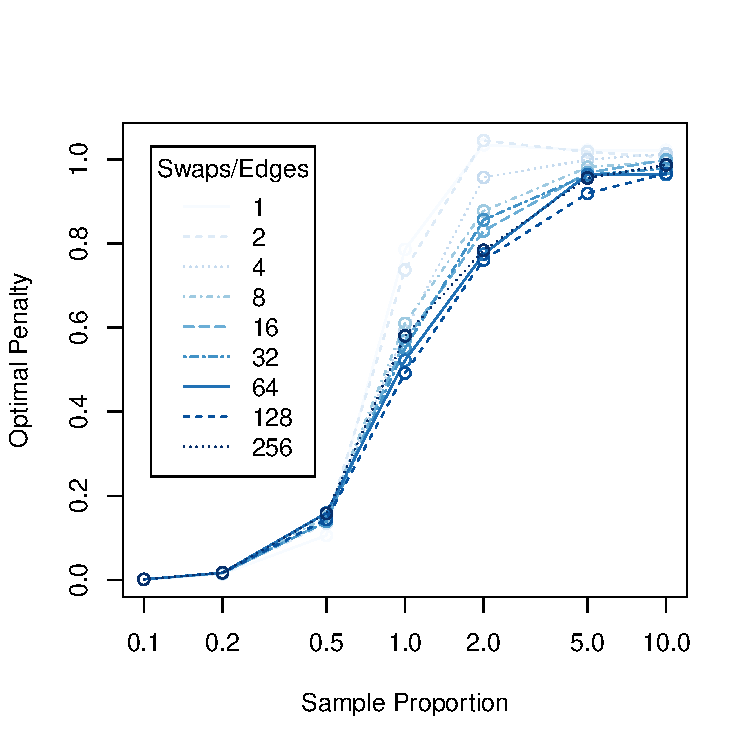
\includegraphics[scale=0.48]{plots/optimal}}
    }
    %\caption{Analytical and emprical priors}
\end{figure}



\section{Concluding remarks}
\label{sxn:conc}

XXX.  BRIEF CONCLUSION HERE.  SOME PHILOSOPHY AND/OR SPECIFIC STATISTICAL LOOSE ENSD THAT WE WANT PEOPLE TO FOLLOW UP ON.



\bibliographystyle{plain}
%\bibliography{refs}
\bibliography{refs,communities,mwmbib_jrnl,mwmbib_proc,mwmbib_book,mwmbib_misc,mwmbib_drft,haribib,communities}

\end{document}
